\documentclass[manuscript=article, journal=jceda8]{achemso}
%\documentclass[journal = jacsat]{achemso}
\usepackage{chemformula} % Formula subscripts using \ch{}
\usepackage[T1]{fontenc} % Use modern font encodings
\usepackage[utf8]{inputenc}
\usepackage[version=3]{mhchem}
\usepackage{gensymb}
\usepackage{upgreek}
\usepackage{pgfplots}
\usepackage{pst-plot}
\usepackage{tikz}
\usepgfplotslibrary{colormaps}
\usetikzlibrary{pgfplots.colormaps}
\usepgfplotslibrary{external} 
\tikzexternalize
\newcommand*\mycommand[1]{\texttt{\emph{#1}}}



\author{András Kiss}
\affiliation{Department of General and Physical Chemistry, University of Pécs, Ifjúság útja 6, 7622 Pécs, Hungary}
\email{akiss@gamma.ttk.pte.hu}
\author{János Klucsik}
\affiliation{Department of General and Physical Chemistry, University of Pécs, Ifjúság útja 6, 7622 Pécs, Hungary}
\author{Géza Nagy}
\affiliation{Department of General and Physical Chemistry, University of Pécs, Ifjúság útja 6, 7622 Pécs, Hungary}
\title{A simple and inexpensive pH electrode made from the tungsten filament of an incandescent light--bulb}
\keywords{pH, electrode, tungsten, light--bulb, potentiometry}



\begin{document}
\begin{abstract}
A simple and robust pH sensitive electrode is presented that can be constructed from cheap and readily available components. The electrode is of the metal/metal--oxide type. The sensing element is the tungsten filament of an incandescent light bulb, whose potential in a solution is dependent on the hydrogen--ion activity. The electrode can be easily built in a high--school chemistry laboratory by students, and can be used to demonstrate the potentiometric determination of pH.
\end{abstract}

\section{Introduction}
pH is one of the most important concepts in chemistry, originally defined by S\o rensen in 1909 \cite{sorensen1909messung} as the negative logarithm of the concentration of hydrogen ion:

\begin{equation}
\textrm{pH} = -\log_{10} c_{\textrm{H}^+}
\end{equation}

At first glance, it looks like a deceptively simple concept. Complications around this definition start to arise when we replace concentration with activity, taking into account that hydrogen ions have charge, therefore their behaviour correlates more closely with activity rather than concentration:

\begin{equation}
\textrm{pH} = -\log_{10} a_{\textrm{H}^+} = -\log_{10} c_{\textrm{H}^+} \gamma_{H^+}
\end{equation}

where $a_{H^+}$ is the activity and $\gamma_{H^+}$ is the activity coefficient of hydrogen ions. This definition however raises a new problem. It includes the activity coefficient of a single ion, which is unmeasurable. Even though the Debye--Hückel equation can be used to calculate a theoretical activity coefficient for a single ion, the prevailing view is that if it cannot be measured, than a pH definition that is based on that activity coefficient is an unmeasurable quantity. This logical difficulty was summarized by Bates and Guggenheim in 1960 \cite{bates1960report}. Their recommended solution was to use 



   might be meaninglesssince it cannot be verified experimentally, Researchers in the late 40s and early 50s solved this problem by defining pH on an instrumental basis, which was summarized by Bates and Guggenheim in 1960 \cite{bates1960report}. Since then, several revisions have been published by IUPAC, the most recent being \cite{covington2002measurement}. The current definition that is described there is based in the \emph{Harned cell}, that is a 

Since then, the definition has been 
Analytical potentiometry started with the discovery and development of the glass pH-electrode. It is the best electrochemical sensor, and one of the best sensors ever made, with a linear response for over more than 13 orders of magnitude, and excellent selectivity.
It was in 1906, when a botanist named Max Cremer discovered that the potential difference across a thin glass membrane is a function of pH when opposite sides of the membrane are in contact with solutions containing different concentrations of H$_3$O$^+$ \cite{cremer1906ursache, cremer1906direkte}.
Three years later, in 1909, S\o rensen introduced the concept of pH \cite{sorensen1909messung}.
He defined it as the negative logarithm of the concentration of H$_3$O$^+$:

\begin{equation}
\textrm{pH} = -\lg c_{\textrm{H}_3\textrm{O}^+}
\end{equation}

This however, is not entirely true, because pH depends on the \emph{activity} of H$_3$O$^+$, rather than its concentration:

\begin{equation}
\textrm{pH} = -\lg a_{\textrm{H}_3\textrm{O}^+}
\end{equation}

And since pH is dimensionless, a better way to define pH is:

\begin{equation}
\textrm{pH} = -\lg(\gamma_{\textrm{H}_3\textrm{O}^+} m_{\textrm{H}_3\textrm{O}^+} / m^\theta)
\end{equation}

or

\begin{equation}
\textrm{pH} = -\lg(\gamma_{\textrm{H}_3\textrm{O}^+} c_{\textrm{H}_3\textrm{O}^+} / c^\theta)
\end{equation}

where $m^\theta$ = 1 mol$\cdot$kg$^{-1}$ and $c^\theta$ = 1 mol$\cdot$dm$^{-3}$ are the standard states, and $\gamma_{\textrm{H}_3\textrm{O}^+}$ is the activity coefficient of H$_3$O$^+$. 

The current, internationally accepted definition of pH is an instrumental definition, based on an electrochemical cell known as the \emph{Harned Cell} \cite{harned1958activity}.
To measure the pH in such a cell, a conventional procedure was developed at NBS (National Bureau of Standards) \cite{durst1975standardization} and recommended at present by the last IUPAC (International Union of Pure and Applied Chemistry) Recommendations \cite{covington2002measurement}.
NIST (National Institute of Standards and Technology) in the U.S. and PTB (Physikalisch-Technische Bundesanstalt) in Germany have presented pH values using the Harned Cell. 

The Harned Cell is described by the following cell diagram: 

\begin{equation}
\textrm{Pt(s) | H}_2\textrm{(g) | buffer solution, Cl}^-\textrm{(aq) | AgCl(s) | Ag(s)}
\label{eq:harned}
\end{equation}

To calculate the potential of the half-cells, the \emph{Nernst-equation} can be used:

\begin{equation}
E = E^\theta - \frac{RT}{z_iF}\ln a_i
\end{equation}

where $E^\theta$ is the standard potential difference of the cell, $R$ the universal gas constant, $F$ the Faraday constant, $T$ the thermodynamic temperature, $z_i$ is the valence and $a_i$ is the activity of ion species $i$.
The potential difference $E$ of the cell \ref{eq:harned} is described by the \emph{Nernst-equation} as:

\begin{equation}
E = E^\theta - \frac{RT\ln 10}{F}\lg\bigg(\frac{a_{\textrm{H}_3\textrm{O}^+}m_{\textrm{Cl}^-}\gamma_{\textrm{Cl}^-}}{m^\theta}\bigg)
\end{equation}

After expressing the pH:

\begin{equation}
\textrm{p}(a_{\textrm{H}_3\textrm{O}^+}\gamma_{\textrm{Cl}^-}) = -\lg(a_{\textrm{H}_3\textrm{O}^+}\gamma_{\textrm{Cl}^-}) = \frac{E - E^\theta}{(RT/F)\ln10} + \lg \bigg(\frac{m_{\textrm{Cl}^-}}{m^\theta}\bigg)
\end{equation}

where $\gamma_{\textrm{Cl}^-}$ is the molal activity coefficient of the chloride ions at the molality $m_{\textrm{Cl}^-}$.

By extrapolating on the equation obtained with least square fitting, the value of the acidity function at zero chloride ion molality p$a_0$ = $-$lg($a_{\textrm{H}^+} \gamma _{\textrm{Cl}^-})m_{\textrm{Cl}^- \to 0}$ can be determined.
Applying the Bates -- Guggenheim convention \cite{bates1960report}, the trace activity coefficient of chloride ions $\gamma_{\textrm{Cl}^- \to 0}$ at $m_{\textrm{Cl}^- \to 0}$ can be calculated:

\begin{equation}
\lg \gamma_{\textrm{Cl}^- \to 0} = \frac{A I^{1/2}}{1 + 1.5I^{1/2}}
\end{equation}

where $A$ is the Debye-Hückel temperature-dependent limiting slope and $I$ the ionic strength of the buffer solution calculated by $I = (1/2) \Sigma c_i z_{i}^{2}$, where $c_i$ and $z_i$ are the molar concentration and electric charge of ionic species $i$.

Haber and Klemensiewicz gave a full account of the response of the glass electrode in their 1909 paper \cite{haber1909elektrische, haber1909concerning}.

There are certain applications where the use of a glass electrode might be challenging or impossible.
These include measuring pH at high temperature or in hydrogen--fluoride solution, or application in the food industry. 

Intensive research has been conducted for several decades to find alternatives to the glass electrode. One such alternative is to use metal/metal-oxide electrodes.
One of the most often used type of these is the Ir/IrO$_2$ electrode \cite{beyenal2004improved}.
The oldest is certainly the Sb/Sb$_2$O$_3$ electrode, its initial characterization dating back to 1923 \cite{uhl1923electrometric}.
It is based on the equilibrium between antimony and the antimony-oxide on its surface.
It is pH sensitive because hydrogen ions participate in the equilibrium:

\begin{equation}
        \ce{2Sb_{(s)} + 3H_2O <=> Sb_2O_3 + 6H^+ + 6e^-}
\end{equation}

\begin{equation}
        \ce{Sb_{(s)} + 3OH^- <=> Sb(OH)_3 + 6e^-}
\end{equation}

Using the Nernst-equation to describe the relationship between [Sb$^{3+}$] and the measured electrode potential \cite{kurzweil2009metal}:

\begin{equation}
E = E^\theta - \frac{RT}{3F}\ln a_{\textrm{Sb}^{3+}}
\end{equation}

Which can be rewritten by using $K_W$, the water ion product, and $K_L$, the solubility product of antimony hydroxide as \cite{kurzweil2009metal}:

\begin{equation}
E = E^\theta - \frac{RT}{3F}\ln \frac{K_L}{K_W} + \frac{RT}{F}\ln a_{\textrm{H}^+}
= E^{\theta '} - \frac{RT}{0.4343F} \textrm{pH}  
\end{equation}
because [Sb$^{3+}$]=[H$^+$]$\cdot K_L / K_W$.

The main reason this particular electrode is so popular is that the melting point of antimony and the softening point of borosilicate glass are similar ($T_{m, \textrm{Sb}} = 630.63~\celsius$, $T_{m, glass}\approx 700~\celsius$), and manufacturing them is relatively easy with standard glass blowing techniques.

Another very popular metal/metal-oxide electrode used for pH measurements is the tungsten electrode. Its function is also based on the equilibrium between the metal and its oxide:
\begin{equation}
        \ce{W_{(s)} + 2H_2O <=> WO_2 + 4H^+ + 4e^-}
\end{equation}




\section{Materials and Methods}

Since tungsten has the highest melting point of all the elements (3422 $\celsius$), the method described in the previous paragraph cannot be used.
A tungsten microwire with a diameter of $30~\upmu$m (Element-explorer, Montreal, Canada) were sealed into a borosilicate glass capillary ($d_i=1.12~$mm, $d_o=2~$mm, no filament, World Precision Inc., Sarasota, Florida, USA).
To seal the microwire, one end of the capillary was closed with flame.
Then, a 1$~$cm long tungsten microwire was inserted from the other end, and pushed down to the sealed end.
The sealed end was melted again while vacuum was being applied from the open end.
The capillary was kept in the flame until $4-5~$mm, about half of the microwire was sealed into the glass.
To make electrical contact between the microwire and the measuring instruments, a small piece of solder was inserted into the capillary.
The solder was melted in flame, and pushed down to the sealed end of the capillary by a sudden shake of the wrist.
While the solder was still melted, a copper wire was insterted into the solder.
After the solder had cooled down, the electrodes were ready to be used.
Microelectrodes with $30~\upmu$m tungsten filaments from a 100$~$W Tungsram incandescent lightbulb were also prepared, using the same method.
Fig. \ref{fig:tungsten_electrode} shows the tip of the finished tungsten microelectrodes.

\begin{figure}
\centering
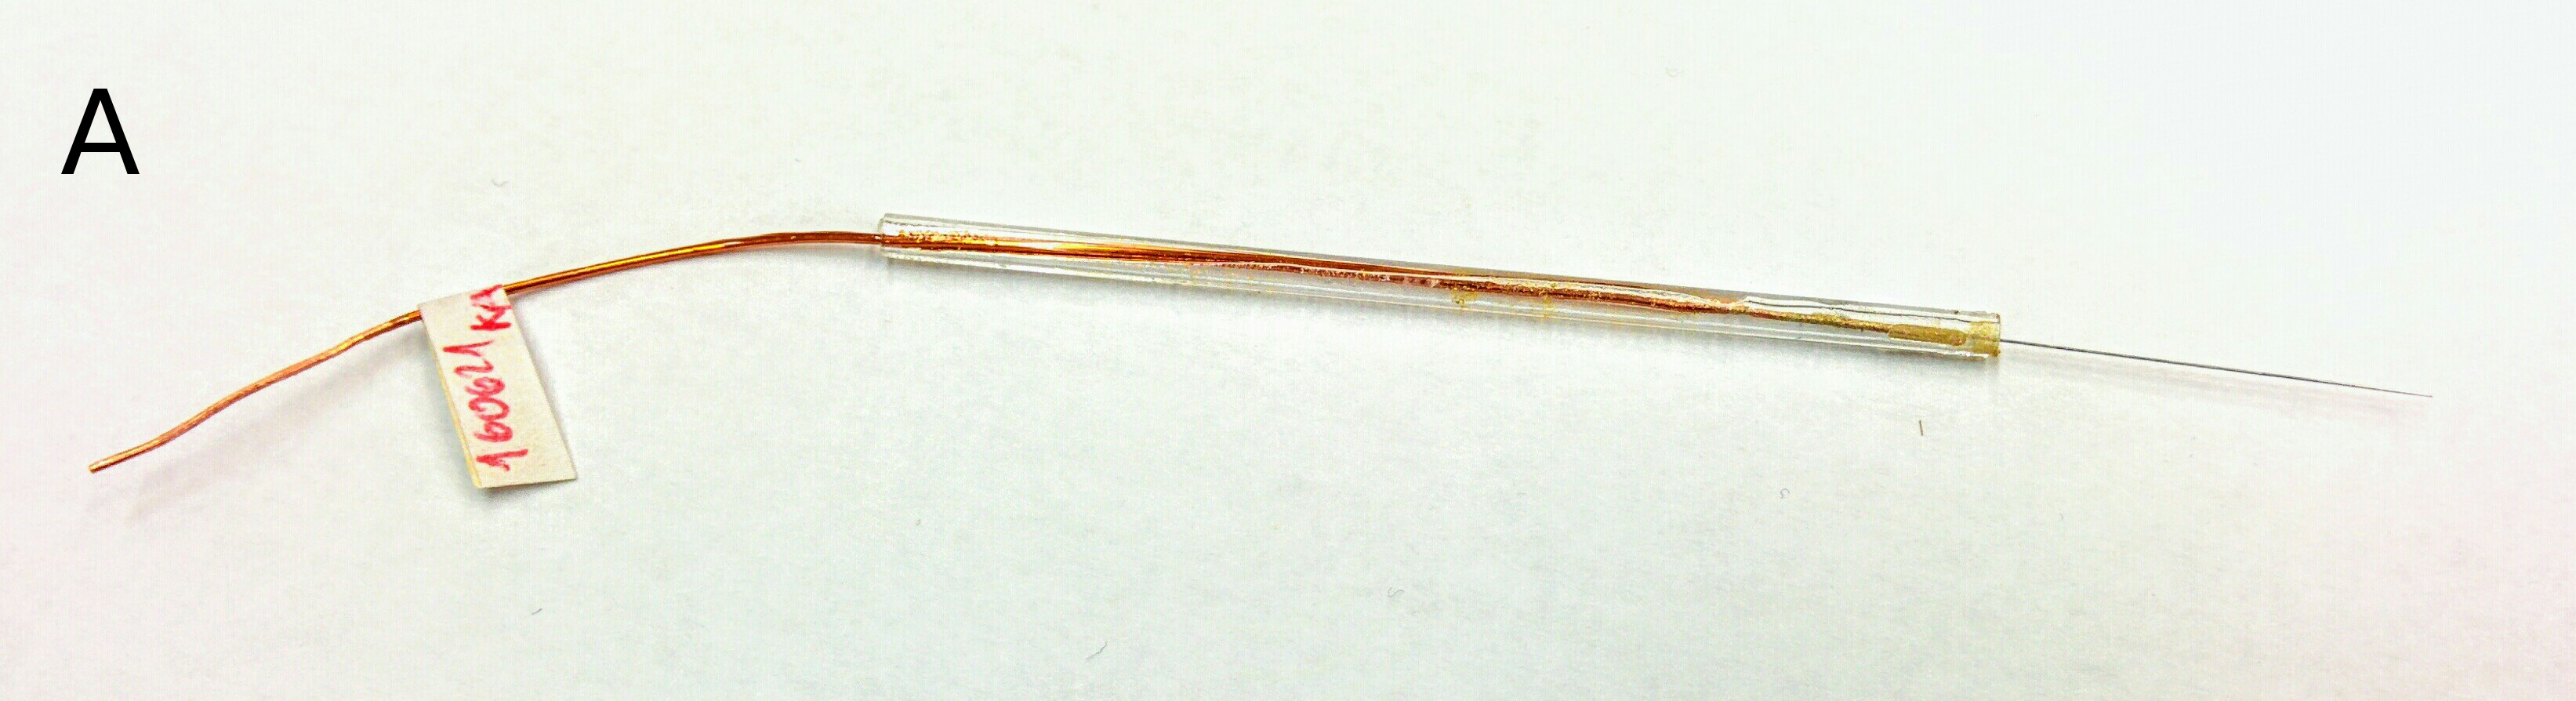
\includegraphics[width=0.9\textwidth]{img/sb_top.jpg}
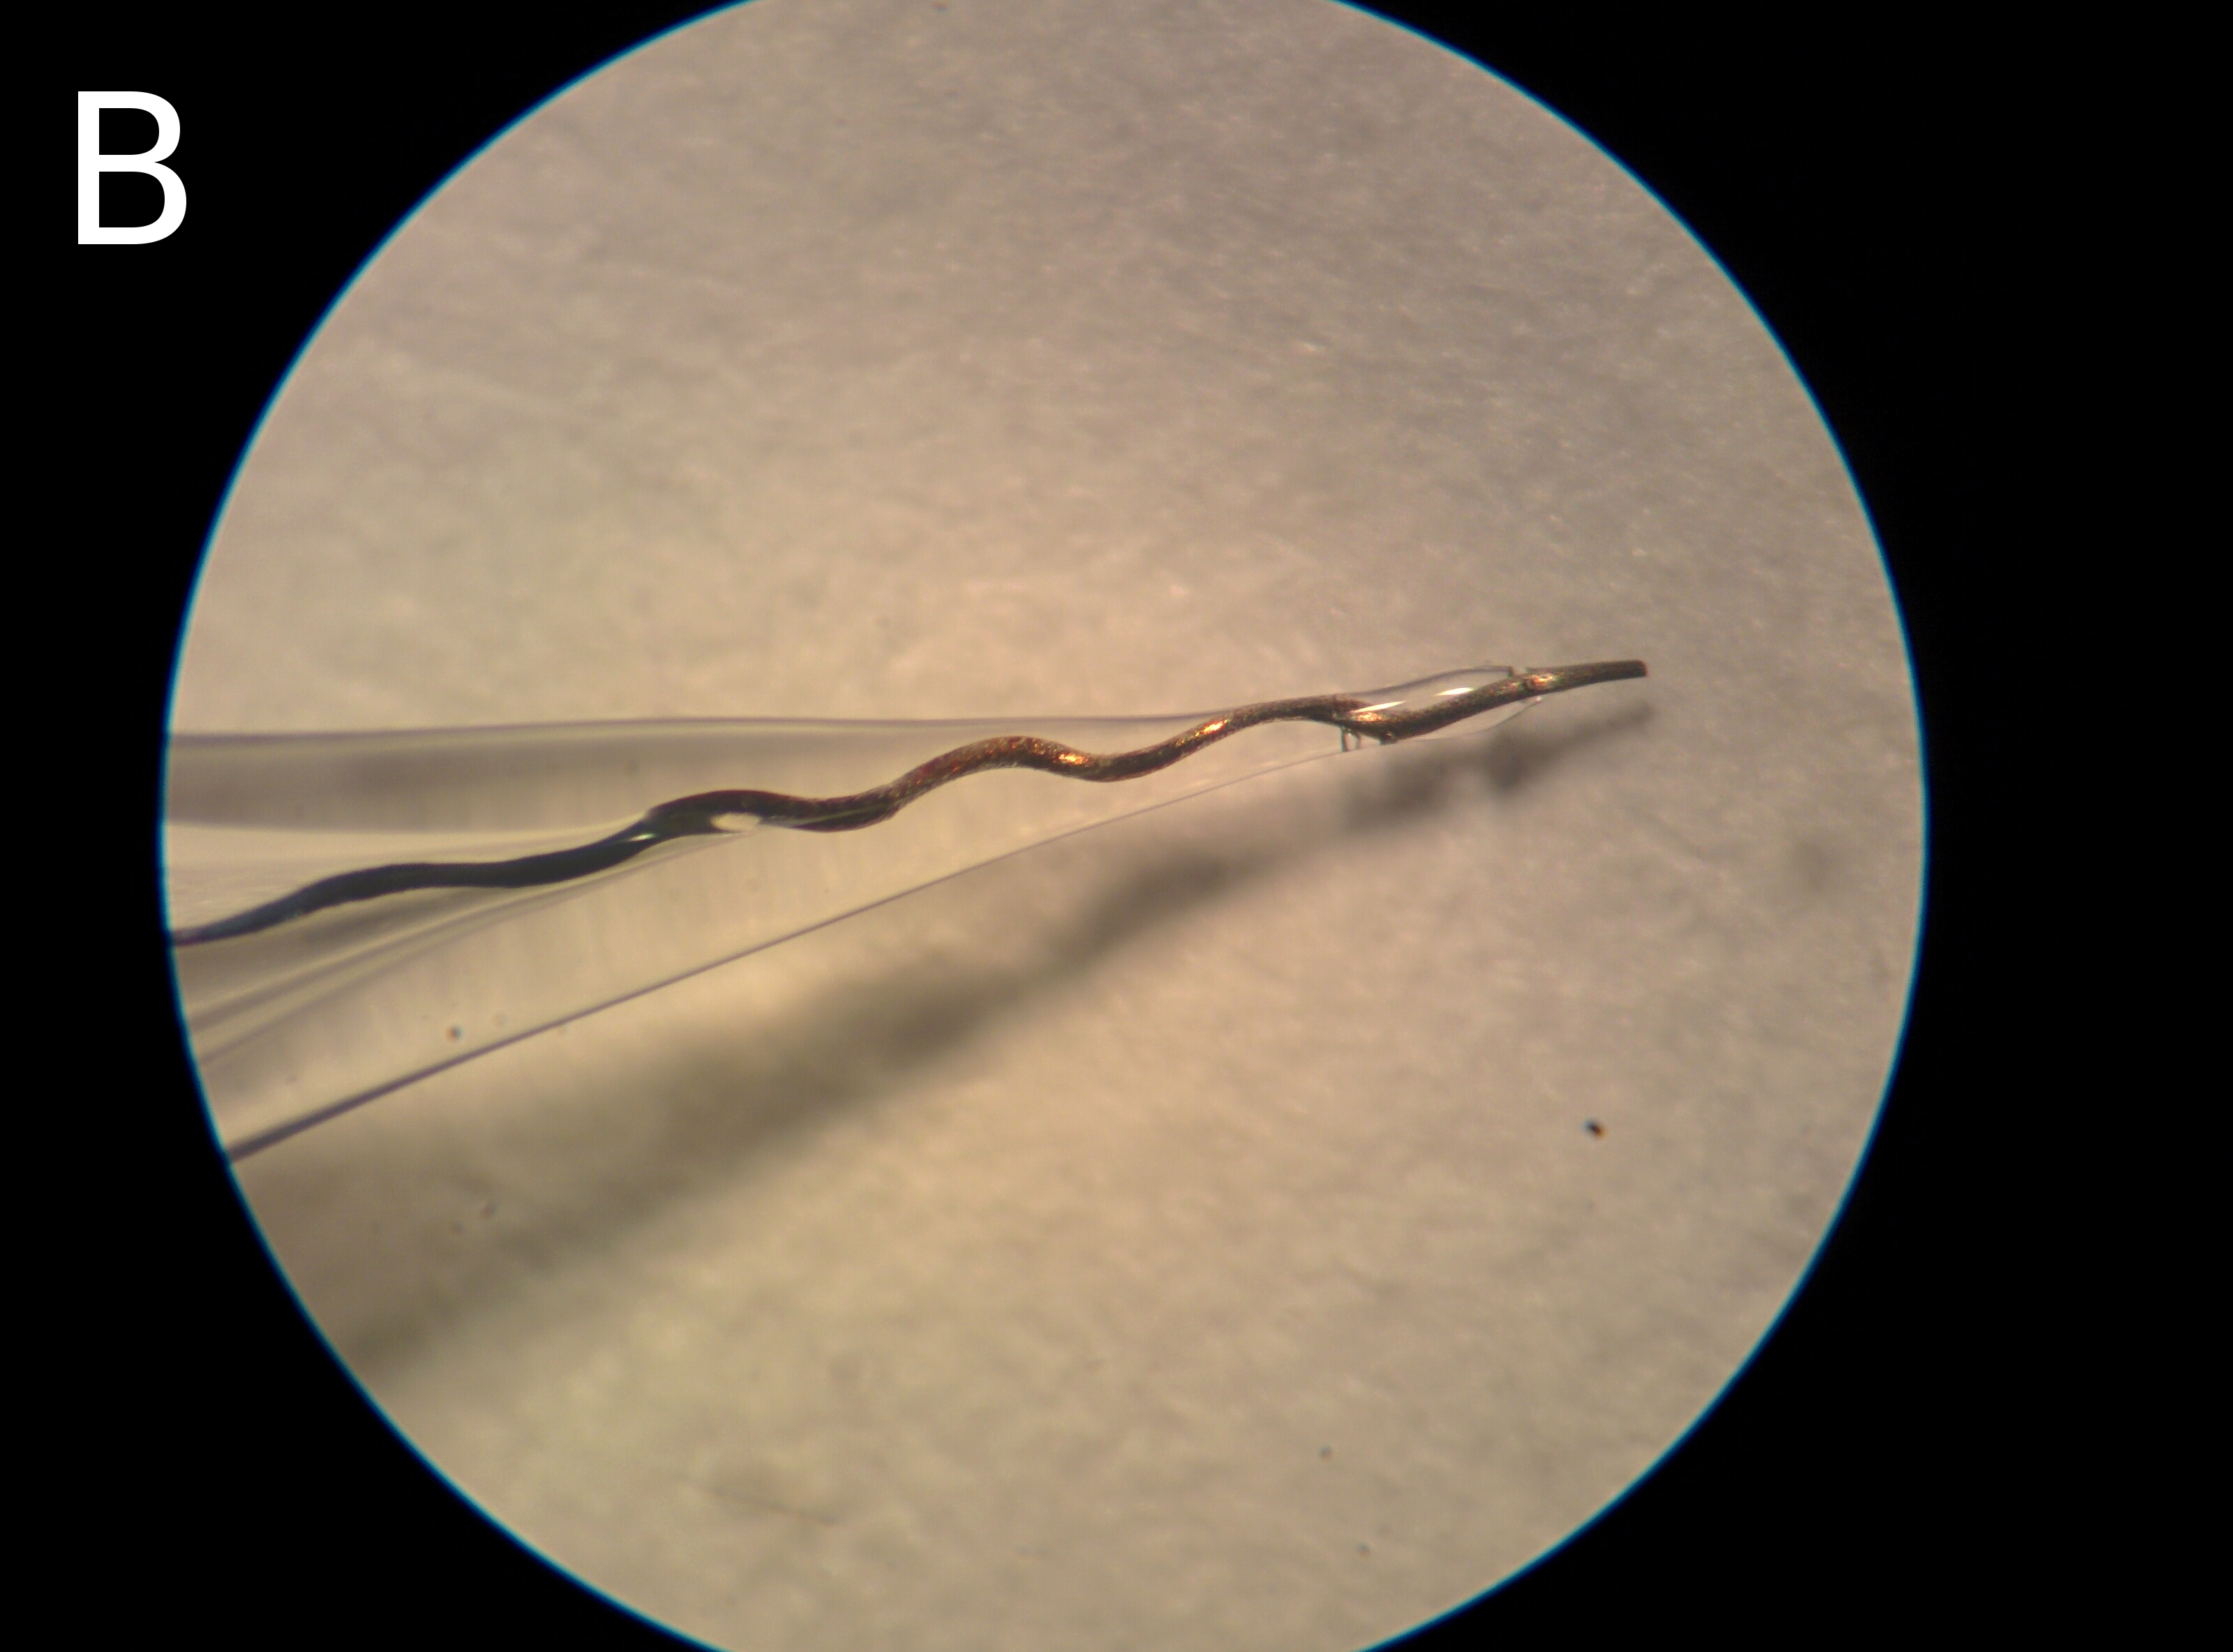
\includegraphics[width=0.45\textwidth]{img/wolfram_electrode1.jpg}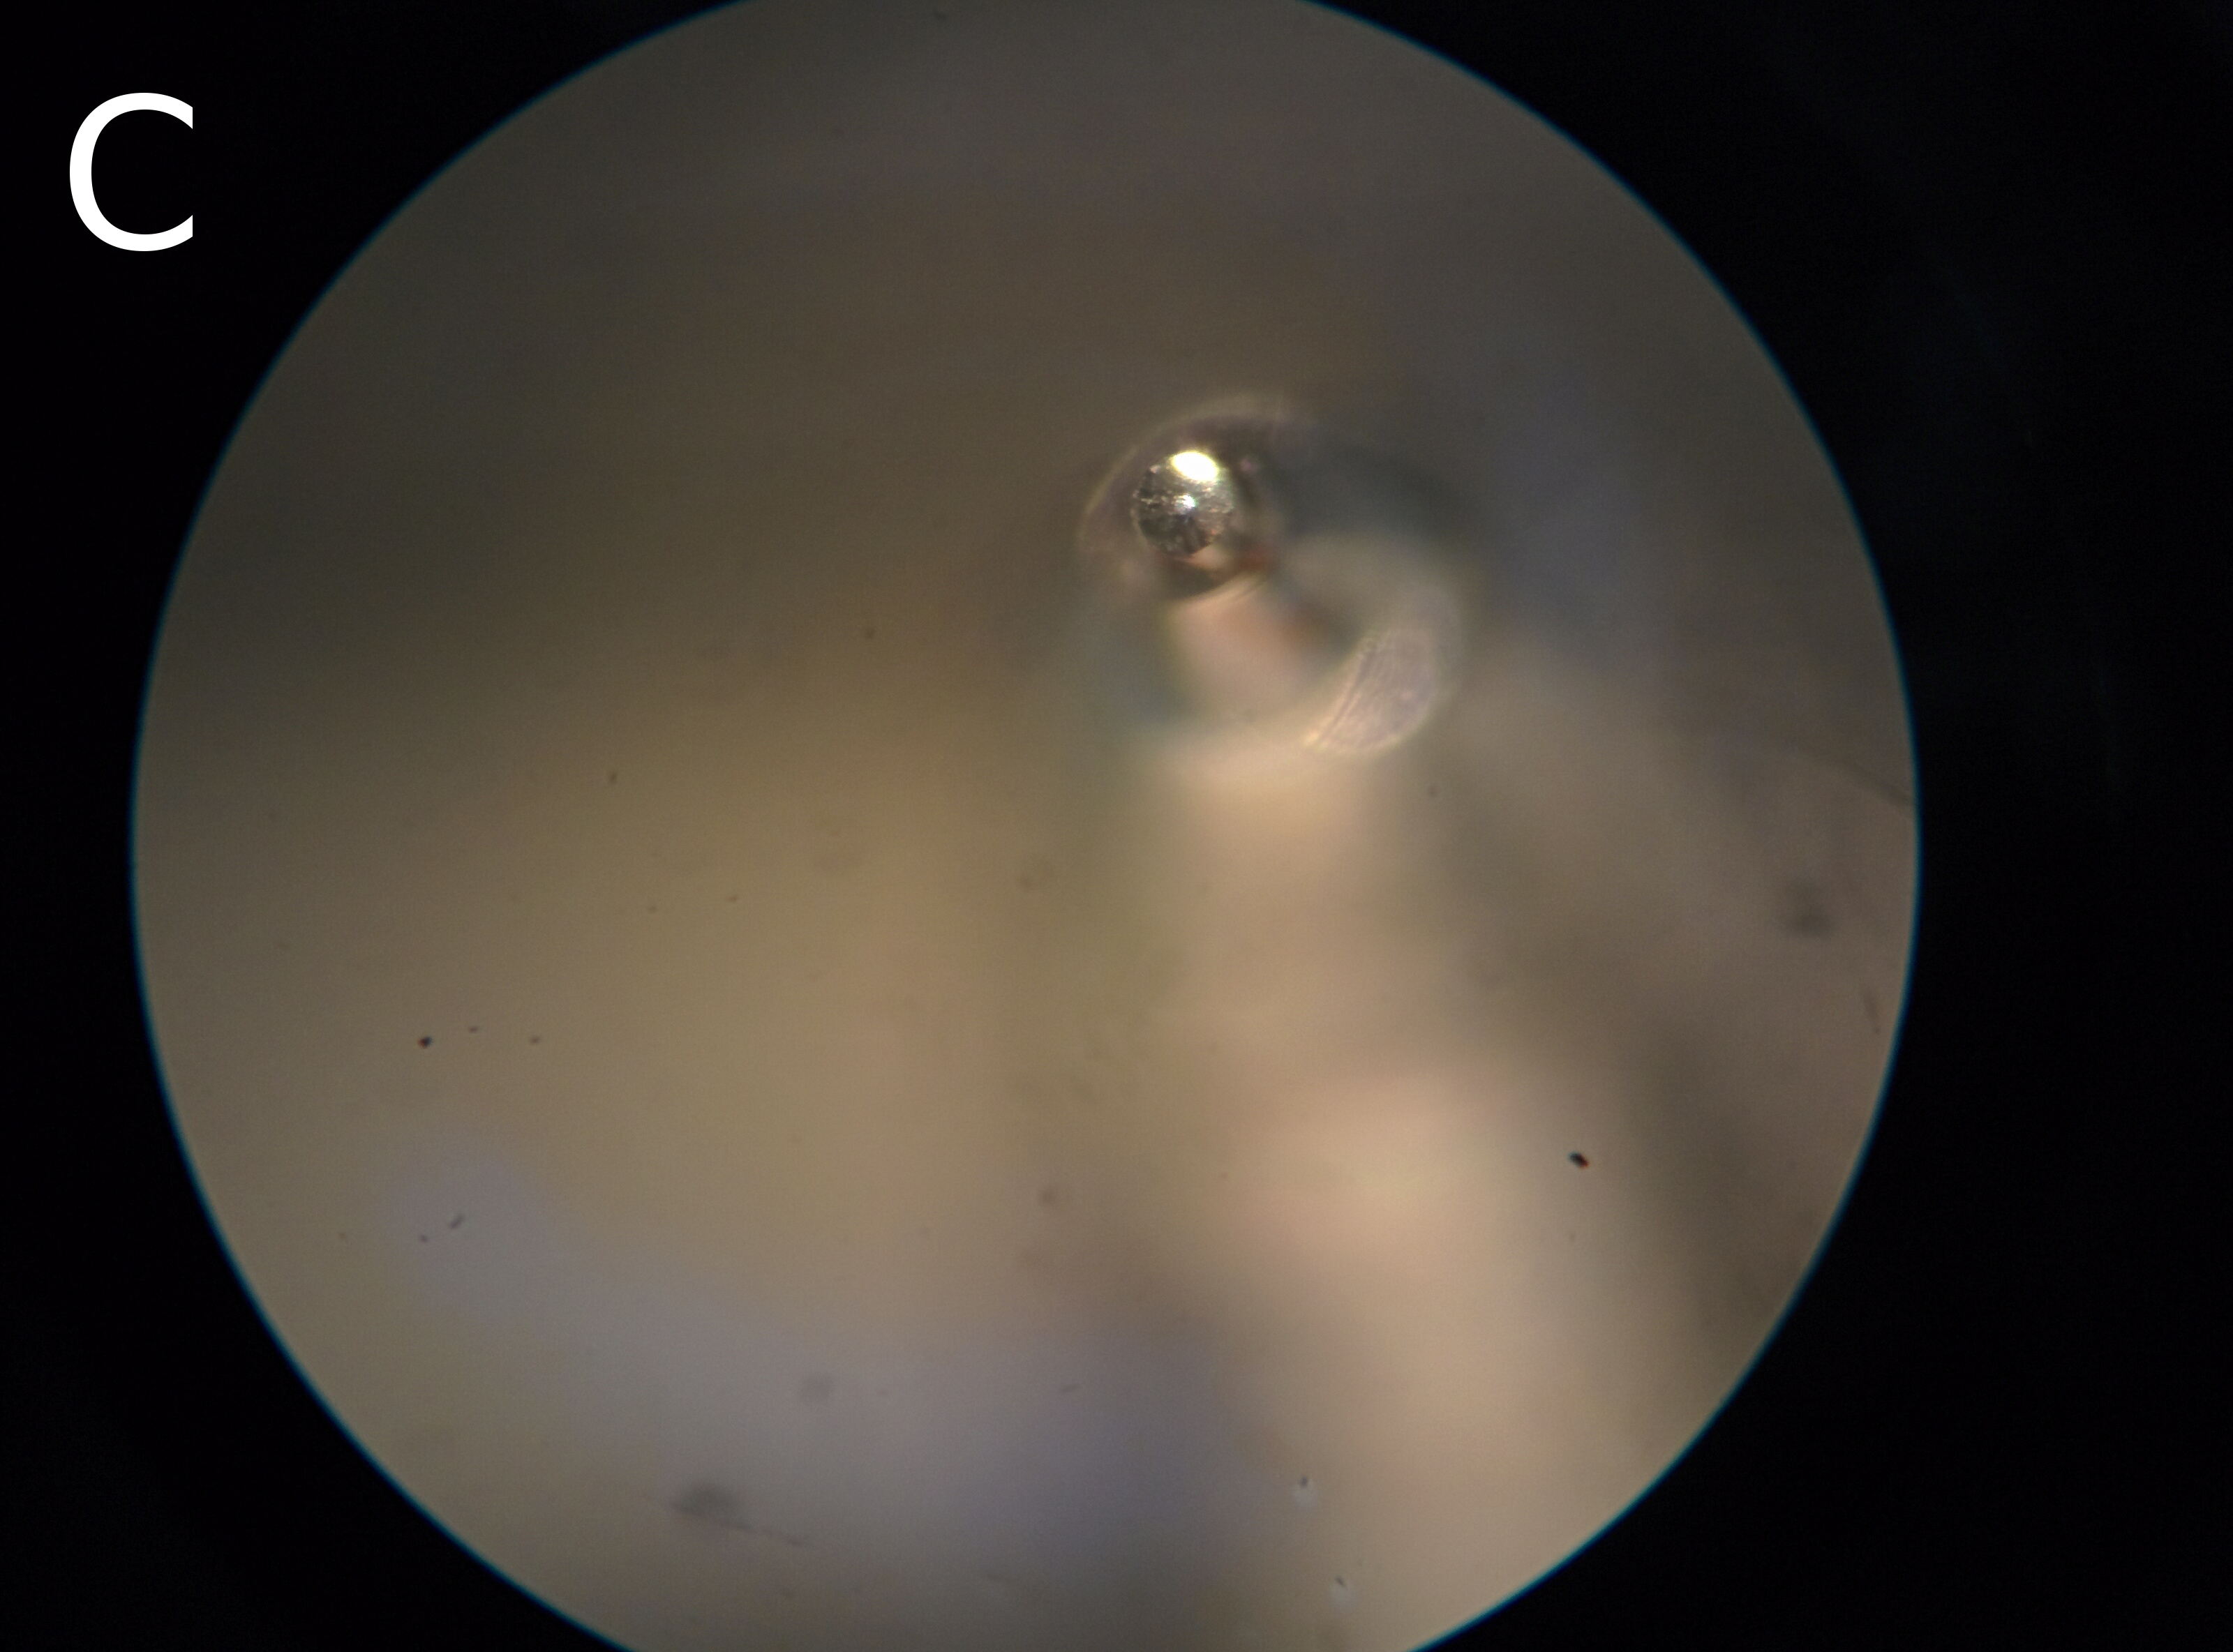
\includegraphics[width=0.45\textwidth]{img/wolfram_electrode2.jpg}

\caption[Antimony and tungsten microelectrodes for local pH measurements.]{(A) Antimony and (B, C) tungsten microelectrodes for local pH measurements.
(B) Side view of the microelectrode prepared from a 100 W Tungsram filament.
(C) Front view of the same electrode.}
\label{fig:tungsten_electrode}
\end{figure}

		
\begin{acknowledgement}
The author thanks Mats Dahlgren for version one of \textsf{achemso},
\end{acknowledgement}

\bibliography{tungsten}
\end{document}
